\documentclass[11pt,a4paper]{article}

% ============ PACKAGES ============
\usepackage[utf8]{inputenc}
\usepackage[T1]{fontenc}
\usepackage[margin=0.8in]{geometry}
\sloppy
\usepackage{amsmath,amssymb}
\usepackage{booktabs}
\usepackage{array}
\usepackage{longtable}
\usepackage{enumitem}
\usepackage{fancyhdr}
\usepackage{hyperref}
\usepackage{xcolor}
\usepackage{tcolorbox}
\tcbuselibrary{breakable}
\usepackage{tikz}
\usetikzlibrary{shapes.geometric, arrows.meta, positioning, calc}

% ============ COLORS ============
\definecolor{codeblue}{rgb}{0.13,0.29,0.53}
\definecolor{layer0}{rgb}{0.8,0.2,0.2}
\definecolor{layer05}{rgb}{0.9,0.4,0.1}
\definecolor{layer1}{rgb}{0.2,0.6,0.2}
\definecolor{layer2}{rgb}{0.2,0.4,0.8}
\definecolor{layer3}{rgb}{0.5,0.2,0.7}
\definecolor{layer6}{rgb}{0.1,0.1,0.1}

% ============ HEADERS ============
\pagestyle{fancy}
\fancyhf{}
\fancyhead[L]{\textit{EFM Codex Map}}
\fancyhead[R]{\thepage}

% ============ HYPERREF ============
\hypersetup{
    colorlinks=true, linkcolor=codeblue, urlcolor=cyan,
    pdftitle={EFM Codex Map},
}

% ============ DOCUMENT ============
\title{
    {\Large\textsc{Entropica Forensic Model}}\\[0.3cm]
    {\LARGE\bfseries Codex Map}\\[0.2cm]
    {\large Crosswalk: Appendices $\Leftrightarrow$ Layers $\Leftrightarrow$ Tests $\Leftrightarrow$ Proofs $\Leftrightarrow$ Clauses}\\[0.3cm]
    {\normalsize Version 1.0}
}
\author{Entropica SPC --- Yology Research Division}
\date{December 2025}

\begin{document}
\maketitle

\begin{abstract}
This document provides a comprehensive crosswalk linking all EFM Codex components: Appendices, Layers, Tests, Proofs, and Constitutional Clauses. It serves as the authoritative reference for traceability across the framework.
\end{abstract}

\tableofcontents
\newpage

%==============================================================================
\section{Visual Architecture Map}
%==============================================================================

\begin{center}
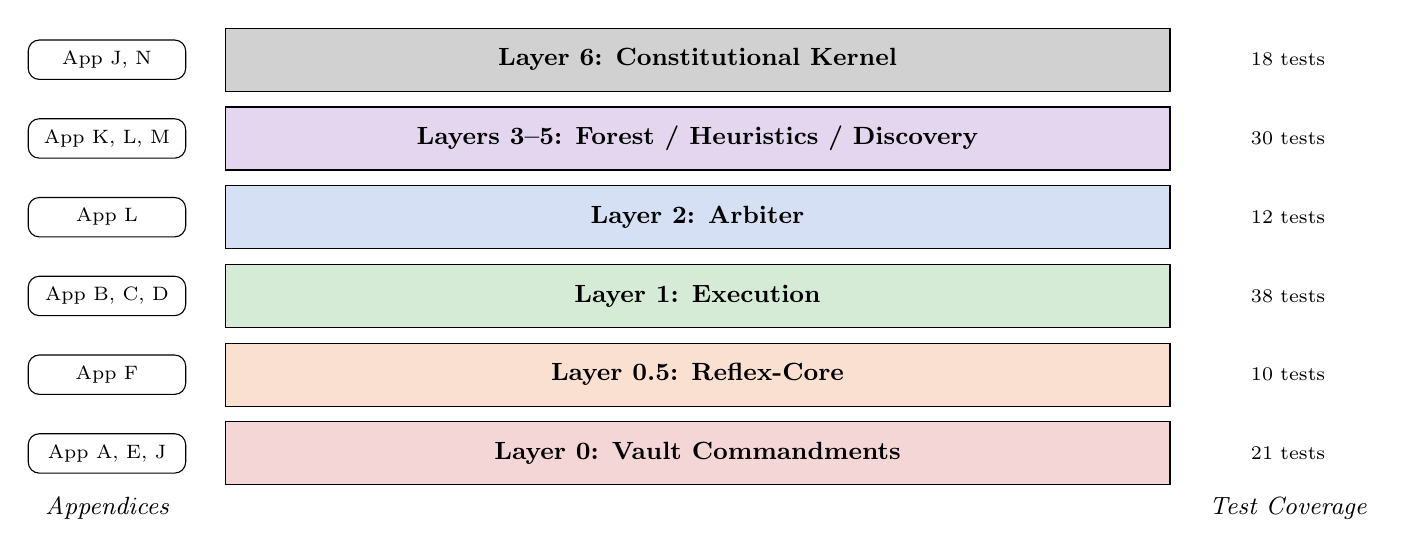
\begin{tikzpicture}[
    layer/.style={rectangle, draw, minimum width=12cm, minimum height=0.8cm, font=\small\bfseries},
    appendix/.style={rectangle, draw, rounded corners, minimum width=2cm, minimum height=0.5cm, font=\scriptsize},
    arrow/.style={->, >=stealth, thick}
]

% Layers
\node[layer, fill=layer6!20] (L6) at (0,6) {Layer 6: Constitutional Kernel};
\node[layer, fill=layer3!20] (L5) at (0,5) {Layers 3--5: Forest / Heuristics / Discovery};
\node[layer, fill=layer2!20] (L2) at (0,4) {Layer 2: Arbiter};
\node[layer, fill=layer1!20] (L1) at (0,3) {Layer 1: Execution};
\node[layer, fill=layer05!20] (L05) at (0,2) {Layer 0.5: Reflex-Core};
\node[layer, fill=layer0!20] (L0) at (0,1) {Layer 0: Vault Commandments};

% Appendix annotations (left side)
\node[appendix, fill=white] at (-7.5,6) {App J, N};
\node[appendix, fill=white] at (-7.5,5) {App K, L, M};
\node[appendix, fill=white] at (-7.5,4) {App L};
\node[appendix, fill=white] at (-7.5,3) {App B, C, D};
\node[appendix, fill=white] at (-7.5,2) {App F};
\node[appendix, fill=white] at (-7.5,1) {App A, E, J};

% Test counts (right side)
\node[font=\scriptsize] at (7.5,6) {18 tests};
\node[font=\scriptsize] at (7.5,5) {30 tests};
\node[font=\scriptsize] at (7.5,4) {12 tests};
\node[font=\scriptsize] at (7.5,3) {38 tests};
\node[font=\scriptsize] at (7.5,2) {10 tests};
\node[font=\scriptsize] at (7.5,1) {21 tests};

% Labels
\node[font=\small\itshape] at (-7.5,0.3) {Appendices};
\node[font=\small\itshape] at (7.5,0.3) {Test Coverage};

\end{tikzpicture}
\end{center}

%==============================================================================
\section{Master Crosswalk Table}
%==============================================================================

\subsection{Layer 0: Vault Commandments}

\begin{longtable}{@{}p{2cm}p{3cm}p{2.5cm}p{2.5cm}p{3cm}@{}}
\toprule
\textbf{Clause} & \textbf{Component} & \textbf{Appendix} & \textbf{Proof} & \textbf{Tests} \\
\midrule
\endhead
C1 & Vault Binding & A §2, J §3 & P4, P5 & A-1, A-2, J-1 \\
C2 & Audit Immutability & E §3, A §4 & P4 & E-1 to E-5 \\
C3 & Reflex Supremacy & F §2, J §4 & P1 & F-1, F-2, V1-2 \\
C4 & Human Override & G §3, J §5 & — & G-1 to G-4 \\
\bottomrule
\end{longtable}

\subsection{Layer 0.5: Reflex-Core}

\begin{longtable}{@{}p{2cm}p{3cm}p{2.5cm}p{2.5cm}p{3cm}@{}}
\toprule
\textbf{Clause} & \textbf{Component} & \textbf{Appendix} & \textbf{Proof} & \textbf{Tests} \\
\midrule
\endhead
R1 & Reflex Gate & F §3 & P1 & F-3, F-4, V1-2 \\
R2 & Micro-Signatures & F §4 & — & F-5, F-6 \\
R3 & Escalation Triggers & F §5 & — & F-7 to F-10 \\
R4 & Cooldown Enforcement & F §6 & P3 & N-1, N-7 \\
\bottomrule
\end{longtable}

\subsection{Layer 1: Execution}

\begin{longtable}{@{}p{2cm}p{3cm}p{2.5cm}p{2.5cm}p{3cm}@{}}
\toprule
\textbf{Clause} & \textbf{Component} & \textbf{Appendix} & \textbf{Proof} & \textbf{Tests} \\
\midrule
\endhead
E1 & Capsule Lifecycle & A §3, D §2 & P5, P6 & A-3, D-1 to D-3 \\
E2 & Spawn Gate & Vol I §4 & P2 & V1-5, V1-7, N-1 \\
E3 & Resource Binding & B §3 & — & B-1 to B-4 \\
E4 & Lexicore Runtime & B §4-5 & — & B-5 to B-8 \\
E5 & DEL Protocol & D §3-4 & — & D-4 to D-6 \\
E6 & Simulation Harness & C §2-5 & — & C-1 to C-24 \\
\bottomrule
\end{longtable}

\subsection{Layer 2: Arbiter}

\begin{longtable}{@{}p{2cm}p{3cm}p{2.5cm}p{2.5cm}p{3cm}@{}}
\toprule
\textbf{Clause} & \textbf{Component} & \textbf{Appendix} & \textbf{Proof} & \textbf{Tests} \\
\midrule
\endhead
A1 & Arbiter Election & L §3 & P7 & V2-1, L-1 \\
A2 & Precedent System & L §4-5 & — & V2-3, L-2 to L-5 \\
A3 & Escalation Routing & L §6 & P7 & V2-2, L-6 \\
A4 & Judicial Swarm & L §7 & — & L-7 to L-12 \\
\bottomrule
\end{longtable}

\subsection{Layers 3--5: Forest / Heuristics}

\begin{longtable}{@{}p{2cm}p{3cm}p{2.5cm}p{2.5cm}p{3cm}@{}}
\toprule
\textbf{Clause} & \textbf{Component} & \textbf{Appendix} & \textbf{Proof} & \textbf{Tests} \\
\midrule
\endhead
F1 & Swarm Health (SHSL) & K §3-5 & P6 & K-1 to K-10 \\
F2 & DCG / SCI & K §6-7 & — & V2-4, V2-5 \\
F3 & Fork / Merge & K §8, J §14 & P8 & V2-6, V2-7, J-8 to J-18 \\
F4 & Discovery Stack & M §3-6 & — & M-1 to M-8 \\
F5 & Dialect Evolution & Vol II §5 & — & V2-12 \\
\bottomrule
\end{longtable}

\subsection{Layer 6: Constitutional Kernel}

\begin{longtable}{@{}p{2cm}p{3cm}p{2.5cm}p{2.5cm}p{3cm}@{}}
\toprule
\textbf{Clause} & \textbf{Component} & \textbf{Appendix} & \textbf{Proof} & \textbf{Tests} \\
\midrule
\endhead
K1 & Genesis Ceremony & J §6 & P8 & J-1, J-2 \\
K2 & Commandment Storage & J §7 & P8 & J-2 \\
K3 & Mutation Protocol & J §8-9 & P8 & J-3, J-4 \\
K4 & Rollback Depth & J §10 & — & J-4 \\
K5 & Gardener Authority & J §11 & — & J-5 \\
K6 & Fork Verification & J §14 & P8 & J-8 to J-18 \\
K7 & ASG Integration & N §3-6 & P2, P3 & N-1 to N-23 \\
\bottomrule
\end{longtable}

%==============================================================================
\section{Property--Proof--Test Matrix}
%==============================================================================

\begin{longtable}{@{}clp{4cm}p{3cm}p{3cm}@{}}
\toprule
\textbf{ID} & \textbf{Property} & \textbf{Definition} & \textbf{Proof Location} & \textbf{Tests} \\
\midrule
\endhead
P1 & Reflex Supremacy & Reflex-Core halts unsafe actions within 1 tick & Vol I §6.1, Testing §2.2 & V1-2, F-1 to F-4 \\
\addlinespace
P2 & Spawn Boundedness & $\forall t: R(t) \leq R_{max}$ & Vol I §6.2, Testing §2.2 & V1-5, N-2, N-5 \\
\addlinespace
P3 & Health Monotonicity & Degradation triggers corrective response & Testing §2.2 & N-1, N-6, K-3 \\
\addlinespace
P4 & Audit Completeness & All transitions logged to d-CTM & Vol I §6.3, Testing §2.2 & E-1 to E-5, N-10 \\
\addlinespace
P5 & Lineage Accountability & Every capsule traceable to genesis & Vol I §6.4, Testing §2.2 & A-1, A-2, V1-4 \\
\addlinespace
P6 & Capsule Liveness & Healthy capsules remain responsive & Testing §2.2 & K-1 to K-5 \\
\addlinespace
P7 & Arbiter Availability & Escalations resolved within bounds & Testing §2.2 & V2-1, V2-2, L-6 \\
\addlinespace
P8 & Constitutional Integrity & Layer 0 preserved across operations & Appendix J §14, Testing §2.2 & J-8 to J-18 \\
\bottomrule
\end{longtable}

%==============================================================================
\section{Appendix--Layer Coverage Matrix}
%==============================================================================

\begin{table}[h]
\centering
\small
\begin{tabular}{@{}l|cccccc|c@{}}
\toprule
\textbf{Appendix} & \textbf{L0} & \textbf{L0.5} & \textbf{L1} & \textbf{L2} & \textbf{L3-5} & \textbf{L6} & \textbf{Tests} \\
\midrule
A: Forensic State & $\bullet$ & & $\bullet$ & & & & 6 \\
B: Lexicore Runtime & & & $\bullet$ & & & & 8 \\
C: Simulation Harness & & & $\bullet$ & $\bullet$ & $\bullet$ & & 24 \\
D: DEL Protocol & & & $\bullet$ & & & & 6 \\
E: ZK-SP Proofs & $\bullet$ & & & & & & 15 \\
F: Escalation Protocol & & $\bullet$ & & & & & 10 \\
G: Gardener Interface & $\bullet$ & & & $\bullet$ & & $\bullet$ & 8 \\
H: Telemetry & & & $\bullet$ & $\bullet$ & $\bullet$ & & 8 \\
I: Deployment Profiles & & & $\bullet$ & & $\bullet$ & $\bullet$ & 6 \\
J: Constitutional Kernel & $\bullet$ & & & & & $\bullet$ & 18 \\
K: SHSL & & & & & $\bullet$ & & 10 \\
L: Judicial Swarms & & & & $\bullet$ & & & 12 \\
M: Discovery Stack & & & & & $\bullet$ & & 8 \\
N: ASG & & & $\bullet$ & & $\bullet$ & $\bullet$ & 23 \\
\midrule
\textbf{Totals} & 4 & 1 & 8 & 4 & 7 & 4 & \textbf{162} \\
\bottomrule
\end{tabular}
\caption{Appendix coverage by layer ($\bullet$ = primary coverage).}
\end{table}

%==============================================================================
\section{Clause ID Reference}
%==============================================================================

Constitutional clauses are identified by layer prefix:

\begin{table}[h]
\centering
\begin{tabular}{@{}lll@{}}
\toprule
\textbf{Prefix} & \textbf{Layer} & \textbf{Range} \\
\midrule
C1--C4 & Layer 0 (Vault) & Four Commandments \\
R1--R4 & Layer 0.5 (Reflex) & Reflex-Core clauses \\
E1--E6 & Layer 1 (Execution) & Execution clauses \\
A1--A4 & Layer 2 (Arbiter) & Arbiter clauses \\
F1--F5 & Layers 3--5 (Forest) & Forest/Heuristic clauses \\
K1--K7 & Layer 6 (Constitutional) & Kernel clauses \\
\bottomrule
\end{tabular}
\caption{Clause ID prefixes by layer.}
\end{table}

%==============================================================================
\section{Test ID Reference}
%==============================================================================

Tests are identified by document prefix:

\begin{table}[h]
\centering
\small
\begin{tabular}{@{}llc@{}}
\toprule
\textbf{Prefix} & \textbf{Document} & \textbf{Count} \\
\midrule
V1-* & Volume I & 8 \\
V2-* & Volume II & 12 \\
A-* & Appendix A & 6 \\
B-* & Appendix B & 8 \\
C-* & Appendix C & 24 \\
D-* & Appendix D & 6 \\
E-* & Appendix E & 15 \\
F-* & Appendix F & 10 \\
G-* & Appendix G & 8 \\
H-* & Appendix H & 8 \\
I-* & Appendix I & 6 \\
J-* & Appendix J & 18 \\
K-* & Appendix K & 10 \\
L-* & Appendix L & 12 \\
M-* & Appendix M & 8 \\
N-* & Appendix N & 23 \\
\midrule
& \textbf{Total} & \textbf{182} \\
\bottomrule
\end{tabular}
\caption{Test ID prefixes by document.}
\end{table}

%==============================================================================
\section{Document Dependency Graph}
%==============================================================================

\begin{center}
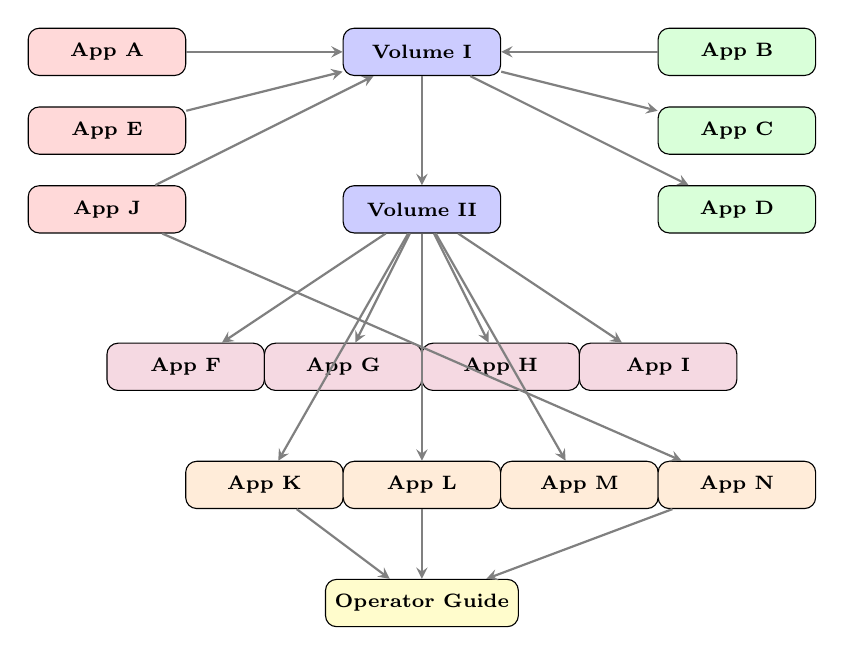
\begin{tikzpicture}[
    doc/.style={rectangle, draw, rounded corners, minimum width=2cm, minimum height=0.6cm, font=\scriptsize\bfseries},
    arrow/.style={->, >=stealth, thick, gray}
]

% Core documents
\node[doc, fill=blue!20] (V1) at (0,4) {Volume I};
\node[doc, fill=blue!20] (V2) at (0,2) {Volume II};

% Appendices - left side (foundations)
\node[doc, fill=red!15] (A) at (-4,4) {App A};
\node[doc, fill=red!15] (E) at (-4,3) {App E};
\node[doc, fill=red!15] (J) at (-4,2) {App J};

% Appendices - right side (runtime)
\node[doc, fill=green!15] (B) at (4,4) {App B};
\node[doc, fill=green!15] (C) at (4,3) {App C};
\node[doc, fill=green!15] (D) at (4,2) {App D};

% Appendices - bottom (governance)
\node[doc, fill=purple!15] (F) at (-3,0) {App F};
\node[doc, fill=purple!15] (G) at (-1,0) {App G};
\node[doc, fill=purple!15] (H) at (1,0) {App H};
\node[doc, fill=purple!15] (I) at (3,0) {App I};

% Appendices - swarm layer
\node[doc, fill=orange!15] (K) at (-2,-1.5) {App K};
\node[doc, fill=orange!15] (L) at (0,-1.5) {App L};
\node[doc, fill=orange!15] (M) at (2,-1.5) {App M};
\node[doc, fill=orange!15] (N) at (4,-1.5) {App N};

% Operator Guide
\node[doc, fill=yellow!20] (OP) at (0,-3) {Operator Guide};

% Arrows
\draw[arrow] (V1) -- (V2);
\draw[arrow] (A) -- (V1);
\draw[arrow] (E) -- (V1);
\draw[arrow] (J) -- (V1);
\draw[arrow] (B) -- (V1);
\draw[arrow] (V1) -- (C);
\draw[arrow] (V1) -- (D);
\draw[arrow] (V2) -- (F);
\draw[arrow] (V2) -- (G);
\draw[arrow] (V2) -- (H);
\draw[arrow] (V2) -- (I);
\draw[arrow] (V2) -- (K);
\draw[arrow] (V2) -- (L);
\draw[arrow] (V2) -- (M);
\draw[arrow] (J) -- (N);
\draw[arrow] (K) -- (OP);
\draw[arrow] (L) -- (OP);
\draw[arrow] (N) -- (OP);

\end{tikzpicture}
\end{center}

%==============================================================================
\section{Code Snippet Index}
%==============================================================================

\begin{longtable}{@{}p{3cm}p{4cm}p{3cm}p{3cm}@{}}
\toprule
\textbf{Snippet} & \textbf{Description} & \textbf{Location} & \textbf{Language} \\
\midrule
\endhead
\texttt{SpawnGate} & Spawn condition validation & Vol I §4.3 & Python \\
\texttt{ReflexEngine} & Millisecond safety response & App F §3.2 & Python \\
\texttt{ZKProofGen} & ZK-SP proof generation & App E §4.1 & Python \\
\texttt{HealthCompute} & Capsule health calculation & App K §4.2 & Python \\
\texttt{ASGCalibrate} & Adaptive spawn calibration & App N §5.1 & Python \\
\texttt{ForkVerifier} & Fork equivalence testing & App J §14.4 & Python \\
\texttt{ArbiterElection} & Arbiter selection protocol & App L §3.3 & Python \\
\texttt{PrecedentLookup} & Judicial precedent retrieval & App L §4.2 & Python \\
\texttt{DialectDistance} & Dialect divergence metric & App K §7.1 & Python \\
\texttt{CapsuleLifecycle} & Lifecycle state machine & App A §3.1 & Python \\
\texttt{d-CTM.append} & Audit log append & App A §4.2 & Python \\
\texttt{GardenerOverride} & Human override handler & App G §3.4 & Python \\
\bottomrule
\caption{Code snippet index across all documents.}
\end{longtable}

%==============================================================================
\section*{Changelog}
%==============================================================================

\textbf{v1.0} (December 2025)
\begin{itemize}[noitemsep]
    \item Initial Codex Map release
    \item Complete crosswalk: 14 appendices, 6 layers, 182 tests, 8 properties
    \item Clause ID reference system established
    \item Code snippet index added
\end{itemize}

\end{document}
